\documentclass[12pt]{article} %***
\usepackage[sectionbib]{natbib}
\usepackage{array,epsfig,fancyheadings,rotating}
\usepackage[]{hyperref}  %<----modified by Ivan
%%%%%%%%%%%%%%%%%%%%%%%%%%%%%%%%%%%%
\usepackage{sectsty, secdot}
%\sectionfont{\fontsize{12}{15}\selectfont}
\sectionfont{\fontsize{12}{14pt plus.8pt minus .6pt}\selectfont}
\renewcommand{\theequation}{\thesection\arabic{equation}}
\subsectionfont{\fontsize{12}{14pt plus.8pt minus .6pt}\selectfont}
%%%%%%%%%%%%%%%%%%%%%%%%%%%%%%%%%%%%%%%%%%%%%%%%%%%%%%%%%%%%%%%%%%%%%%%%%%%%%%%%%%%%%%%%

\textwidth=31.9pc
\textheight=46.5pc
\oddsidemargin=1pc
\evensidemargin=1pc
\headsep=15pt
%\headheight=.2cm
\topmargin=.6cm
\parindent=1.7pc
\parskip=0pt

\usepackage{amsmath}
\usepackage{amssymb}
\usepackage{amsfonts}
\usepackage{multirow}
\usepackage{amsthm}

\setcounter{page}{1}
\newtheorem{theorem}{Theorem}
\newtheorem{lemma}{Lemma}
\newtheorem{corollary}{Corollary}
\newtheorem{proposition}{Proposition}
\theoremstyle{definition}
\newtheorem{definition}{Definition}
%\newtheorem{proof}{Proof}
\newtheorem{example}{Example}
\newtheorem{remark}{Remark}
\pagestyle{fancy}

%%%%%%%%%%%%%%%%%%%%%%%%%%%%%%%%%%%%%%%%%%%%%%%%%%%%%%%%%%%%%%%%%%%%%%%%%%%%%%%%%%%%%%%%%%%%%%%%%%%%%%%%%%%%%%%%%%%%%%%%%%%%
\pagestyle{fancy}
\def\n{\noindent}
\lhead[\fancyplain{} \leftmark]{}
\chead[]{}
\rhead[]{\fancyplain{}\rightmark}
\cfoot{}
%\headrulewidth=0pt  %<-modified by Ivan

%%%%%%%%%%%%%%%%%%%%%%%%%%%%%%%%%%%%%%%%%%%%%%%%%%%%%%%%%%%%%%%%%%%%%%%%%%%%%%%%%%%%%%%%%%%%%%%%%%%%%%%%%%%%%%%%%%%%%%%%%%%%
%%%%%%%%%%%%%%%%%%%%%%%%%%%%%%%%%%%%%%%%%%%%%%%%%%%%%%%%%%%%%%%%%%%%%%%%%%%%%%%%%%%%%%%%%%%%%%%%%%%%%%%%%%%%%%%%%%%%%%%%%%%%

\begin{document}
	
	%%%%%%%%%%%%%%%%%%%%%%%%%%%%%%%%%%%%%%%%%%%%%%%%%%%%%%%%%%%%%%%%%%%%%%%%%%%%%%%%%%%%%%%%%%%%%%%%%%%%%%%%%%%%%%%%%%%%%%%%%%%%
	%%%%%%%%%%%%%%%%%%%%%%%%%%%%%%%%%%%%%%%%%%%%%%%%%%%%%%%%%%%%%%%%%%%%%%%%%%%%%%%%%%%%%%%%%%%%%%%%%%%%%%%%%%%%%%%%%%%%%%%%%%%%
	
	\renewcommand{\baselinestretch}{2}
	
	\markright{ \hbox{\footnotesize\rm Statistica Sinica
			%{\footnotesize\bf 24} (201?), 000-000
		}\hfill\\[-13pt]
		\hbox{\footnotesize\rm
			%\href{http://dx.doi.org/10.5705/ss.20??.???}{doi:http://dx.doi.org/10.5705/ss.20??.???}
		}\hfill }
	
	\markboth{\hfill{\footnotesize\rm FIRSTNAME1 LASTNAME1 AND FIRSTNAME2 LASTNAME2} \hfill}
	{\hfill {\footnotesize\rm FILL IN A SHORT RUNNING TITLE} \hfill}
	
	\renewcommand{\thefootnote}{}
	$\ $\par
	
	%%%%%%%%%%%%%%%%%%%%%%%%%%%%%%%%%%%%%%%%%%%%%%%%%%%%%%%%%%%%%%%%%%%%%%%%%%%%%%%%%%%%%%%%%%%%%%%%%%%%%%%%%%%%%%%%%%%%%%%%%%%%
	
	\fontsize{12}{14pt plus.8pt minus .6pt}\selectfont \vspace{0.8pc}
	\centerline{\large\bf TITLE OF THE ARTICLE FIRST LINE UP TO }
	\vspace{2pt} 
	\centerline{\large\bf HERE IF A SECOND LINE IS NEEDED}
	\vspace{.4cm} 
	\centerline{Author(s)} 
	\vspace{.4cm} 
	\centerline{\it Affiliation(s)}
	\vspace{.55cm} \fontsize{9}{11.5pt plus.8pt minus.6pt}\selectfont
	
	%%%%%%%%%%%%%%%%%%%%%%%%%%%%%%%%%%%%%%%%%%%%%%%%%%%%%%%%%%%%%%%%%%%%%%%%%%%%%%%%%%%%%%%%%%%%%%%%%%%%%%%%%%%%%%%%%%%%%%%%%%%%
	
	\begin{quotation}
		\noindent {\it Abstract:}
		{\bf Contents of the Abstract.}\\
		Lorem ipsum dolor sit amet, debet putant in nec, fugit gloriatur eloquentiam no vix. Hinc mucius disputando sit ad. Qui quas ubique ancillae id. Ad mel doctus tacimates, vis fabellas interesset ei.
		Nam tamquam prompta omittantur no. Te oratio liberavisse ius. Quo ea eruditi fierent, dicant exerci forensibus mel ex. Quod clita scripta ea his, in sea semper prompta inciderint. Eam ut mundi mnesarchum. Cum illud augue sonet eu.
		In usu dicat choro putent, no atqui viderer eleifend nec. Ei mea cibo senserit. Consul dissentiunt sea ei. Et discere scriptorem quo. Agam nonumy eirmod no vim, cu per odio abhorreant.
		Sit id scripta delenit, ad stet fierent nam, ex sale qualisque qui. Ei animal invidunt consulatu vis, cu vel decore euismod. Eos et autem altera, per ex quem nibh praesent. Vix te vide deseruisse, est justo possit iuvaret cu.
		Usu eripuit repudiare ne. Nobis oportere salutatus qui ex. Has eu quando appellantur mediocritatem, sit no regione singulis. Ei nibh idque sed, in libris voluptaria mea.
		
		
		\vspace{9pt}
		\noindent {\it Key words and phrases:}
		Balanced incomplete block design, Hadamard matrix, nearly balanced incomplete block design, orthogonal array.
		\par
	\end{quotation}\par
	
	
	
	\def\thefigure{\arabic{figure}}
	\def\thetable{\arabic{table}}
	
	\renewcommand{\theequation}{\thesection.\arabic{equation}}
	
	
	\fontsize{12}{14pt plus.8pt minus .6pt}\selectfont
	
	
	
	
	
	\section{ The First Section}
	
	{\it Statistica Sinica} uses {\bf natbib} package, and here are some examples of using {\bf natbib} packages:
	\cite{1988},
	Contents of the first section.\\
	\citet[Chap.~2]{1943}.
	Contents of the first section.\\
	\cite{Eubank}.
	Contents of the first section.\\
	\cite{Noakes}.
	Contents of the first section.\\
	
	\par
	
	\begin{equation}\label{1.1}
	\mbox {The 1st display equation of the first section.}
	\end{equation}
	\begin{equation}\label{1.2}
	\mbox {The 2nd display equation of the first section.}
	\end{equation}
	
	
	Lorem ipsum dolor sit amet (\citet{Noakes, Eubank}), debet putant in nec, fugit gloriatur eloquentiam no vix. Hinc mucius disputando sit ad. Qui quas ubique ancillae id. Ad mel doctus tacimates, vis fabellas interesset ei.
	Nam tamquam prompta omittantur no. Te oratio liberavisse ius. Quo ea eruditi fierent, dicant exerci forensibus mel ex. Quod clita scripta ea his, in sea semper prompta inciderint. Eam ut mundi mnesarchum. Cum illud augue sonet eu.
	In usu dicat choro putent, no atqui viderer eleifend nec. Ei mea cibo senserit. Consul dissentiunt sea ei. Et discere scriptorem quo. Agam nonumy eirmod no vim, cu per odio abhorreant.
	Sit id scripta delenit, ad stet fierent nam, ex sale qualisque qui. Ei animal invidunt consulatu vis, cu vel decore euismod. Eos et autem altera, per ex quem nibh praesent. Vix te vide deseruisse, est justo possit iuvaret cu.
	Usu eripuit repudiare ne. Nobis oportere salutatus qui ex. Has eu quando appellantur mediocritatem, sit no regione singulis. Ei nibh idque sed, in libris voluptaria mea.
	\begin{theorem}
		Contents of the Theorem.\\
		Lorem ipsum dolor sit amet, debet putant in nec, fugit gloriatur eloquentiam no vix. Hinc mucius disputando sit ad. Qui quas ubique ancillae id. Ad mel doctus tacimates, vis fabellas interesset ei.
	\end{theorem}
	
	
	
	
	\section{The Second Section}
	{\bf Contents of the second section.}
	\cite{1943}, Lorem ipsum dolor sit amet, debet putant in nec, fugit gloriatur eloquentiam no vix. Hinc mucius disputando sit ad. Qui quas ubique ancillae id. Ad mel doctus tacimates, vis fabellas interesset ei.
	Nam tamquam prompta omittantur no. Te oratio liberavisse ius. Quo ea eruditi fierent, dicant exerci forensibus mel ex. Quod clita scripta ea his, in sea semper prompta inciderint. Eam ut mundi mnesarchum. Cum illud augue sonet eu.
	In usu dicat choro putent, no atqui viderer eleifend nec. Ei mea cibo senserit. Consul dissentiunt sea ei. Et discere scriptorem quo. Agam nonumy eirmod no vim, cu per odio abhorreant.
	Sit id scripta delenit, ad stet fierent nam, ex sale qualisque qui. Ei animal invidunt consulatu vis, cu vel decore euismod. Eos et autem altera, per ex quem nibh praesent. Vix te vide deseruisse, est justo possit iuvaret cu.
	Usu eripuit repudiare ne. Nobis oportere salutatus qui ex. Has eu quando appellantur mediocritatem, sit no regione singulis. Ei nibh idque sed, in libris voluptaria mea.
	
	
	
	\begin{figure}[t!]
		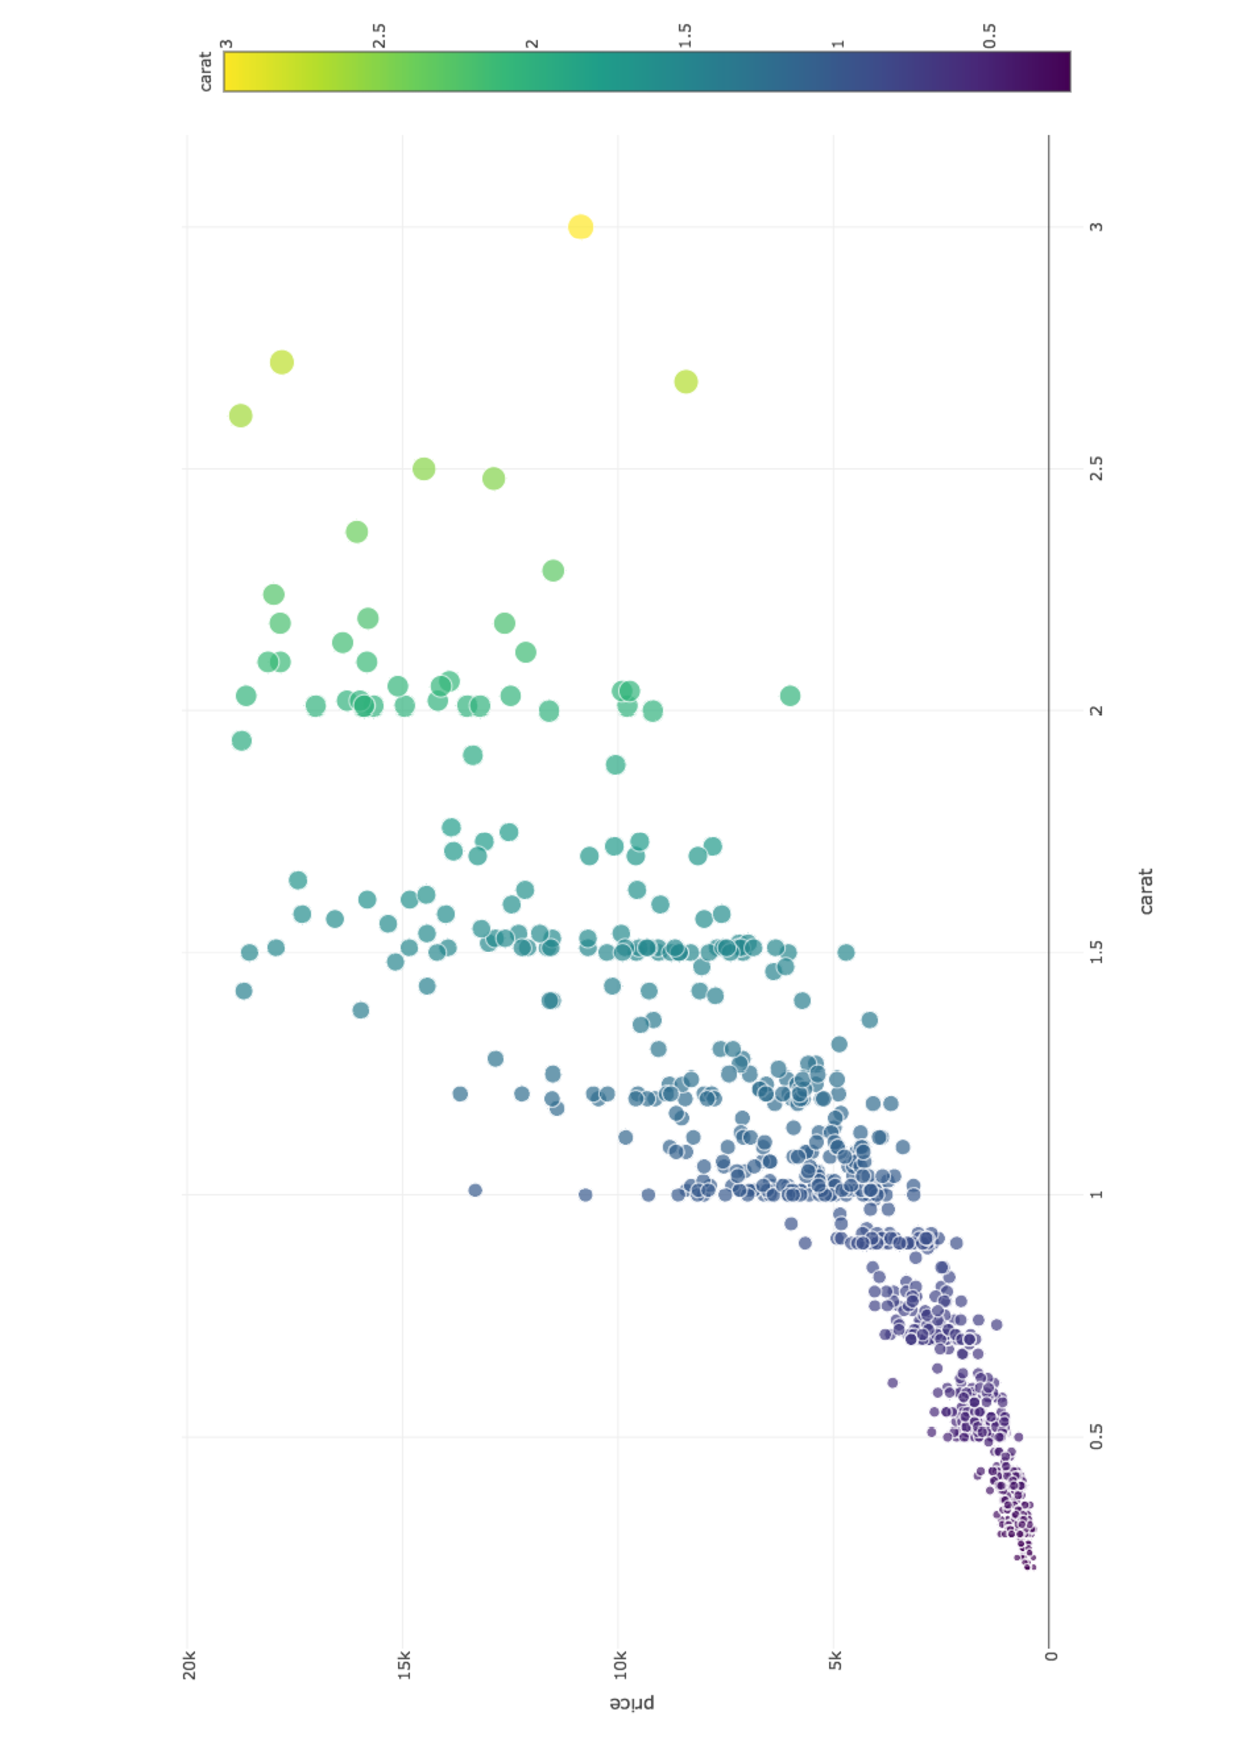
\includegraphics [angle=-90, scale=0.45]{carat}\par
		%\centerline{\epsfig{file=d:/sinicas/simuh3.eps,angle=-90,width=4.5in}}\par
		%\centerline{\epsfig{file=d:/sinicas/simuh4.eps,width=4.5in}}\par
		%\centerline{\epsfig{file=logo.eps,width=4.5in}}\par  %<- modified by Ivan  (You need to put figure in the same folder; or you must specify the path to the figure.)
		\caption{Caption of the figure.}
	\end{figure}
	
	\begin{equation}\label{2.1}
	\mbox {The 1st display equation of the second section.}
	\end{equation}
	\begin{equation}\label{2.2}
	\mbox {The 2nd display equation of the second section.}
	\end{equation}
	
	%%%%%%%%%%%%%%%%%%%%%%%%%%%%%%%%%%%%%%%%%%%%%%%%%%%%%%%%%%%%%%%%%%%%%%%%%%%%%%%%%%%%%%%%%%%%%%%%%%%%%%%%%%%%%%%%%%%%%%%%%%%%
	
	
	\section{The Third Section}
	{\bf Contents of the third section.}\\
	Lorem ipsum dolor sit amet, debet putant in nec, fugit gloriatur eloquentiam no vix. Hinc mucius disputando sit ad. Qui quas ubique ancillae id. Ad mel doctus tacimates, vis fabellas interesset ei.
	Nam tamquam prompta omittantur no. Te oratio liberavisse ius. Quo ea eruditi fierent, dicant exerci forensibus mel ex. Quod clita scripta ea his, in sea semper prompta inciderint. Eam ut mundi mnesarchum. Cum illud augue sonet eu.
	In usu dicat choro putent, no atqui viderer eleifend nec. Ei mea cibo senserit. Consul dissentiunt sea ei. Et discere scriptorem quo. Agam nonumy eirmod no vim, cu per odio abhorreant.
	Sit id scripta delenit, ad stet fierent nam, ex sale qualisque qui. Ei animal invidunt consulatu vis, cu vel decore euismod. Eos et autem altera, per ex quem nibh praesent. Vix te vide deseruisse, est justo possit iuvaret cu.
	Usu eripuit repudiare ne. Nobis oportere salutatus qui ex. Has eu quando appellantur mediocritatem, sit no regione singulis. Ei nibh idque sed, in libris voluptaria mea.
	
	
	Contents of the third section.
	\begin{equation}\label{3.1}
	\mbox {The 1st display equation of the third section.}
	\end{equation}
	\begin{equation}\label{3.2}
	\mbox {The 2nd display equation of the third section.}
	\end{equation}
	\newpage
	\begin{table}[t!] %***
		\caption{Caption of the table.}
		\label{tab:simulation}\par
		\resizebox{\linewidth}{!}{\begin{tabular}{|rcrrrrrrrrr|} \hline %***5truept
				\multicolumn{2}{|c}{Bandwidth}
				& \multicolumn{3}{c}{$h=3$}
				& \multicolumn{3}{c}{$h=4$}
				& \multicolumn{3}{c|}{$h=5$} \\ \hline
				\multicolumn{2}{|c}{Estimates}
				& \multicolumn{1}{c}{$\hat N_H^{LC}$} & \multicolumn{1}{c}{$\hat N_{\bar H}^{LC}$} & \multicolumn{1}{c}{$\hat N_{\bar H}^{LL}$}
				& \multicolumn{1}{c}{$\hat N_H^{LC}$} & \multicolumn{1}{c}{$\hat N_{\bar H}^{LC}$} & \multicolumn{1}{c}{$\hat N_{\bar H}^{LL}$}
				& \multicolumn{1}{c}{$\hat N_H^{LC}$} & \multicolumn{1}{c}{$\hat N_{\bar H}^{LC}$} & \multicolumn{1}{c|}{$\hat N_{\bar H}^{LL}$} \\[3pt] \hline
				$beta(10,10)$ & BIAS  &-22.5&-14.8&14.0&-13.3&-6.9&12.5&-8.2&-4.7&11.5 \\
				$\bar{p}=0.500$ & S.E. &13.8&14.9&12.1&12.6&14.6&11.7&15.1&19.3&15.5 \\
				$cv=0.218$ & RMSE &26.4&21.0&18.5&18.3&16.2&17.1&17.2&19.9&19.3
				\\ \hline
				$beta(5,5)$ & BIAS &-32.2&-19.9&5.4&-21.9&-11.8&4.9&-15.6&-8.4&5.1 \\
				$\bar{p}=0.500$ & S.E. &15.8&16.2&12.3&14.3&19.8&12.9&16.4&19.8&14.6 \\
				$cv=0.302$ & RMSE &35.9&25.7&13.4&26.1&15.9&11.9&22.6&21.5&15.4
				\\ \hline
				$beta(4,8)$ & BIAS &-53.7&-29.1&-10.8&-42.0&-19.3&-8.4&-34.4&-13.9&-7.6 \\
				$\bar{p}=0.333$ & S.E. &20.8&19.4&18.1&18.5&18.8&15.6&19.2&20.6&16.4 \\
				$cv=0.392$ & RMSE &57.6&34.9&21.1&45.9&26.9&17.8&39.4&24.9&18.1
				\\ \hline
				$beta(3,5)$ & BIAS &-57.4&-32.4&-15.5&-45.6&-22.8&-13.1&-37.4&-17.1&-11.4 \\
				$\bar{p}=0.375$ & S.E. &21.2&19.9&17.1&18.9&18.8&15.0&19.6&21.6&15.6 \\
				$cv=0.430$ & RMSE &61.2&38.1&23.1&49.4&29.5&19.9&42.3&27.5&19.3
				\\ \hline
		\end{tabular}}
	\end{table}
	
	\section{Fourth Section}
	Lorem ipsum dolor sit amet, debet putant in nec, fugit gloriatur eloquentiam no vix. Hinc mucius disputando sit ad. Qui quas ubique ancillae id. Ad mel doctus tacimates, vis fabellas interesset ei.
	Nam tamquam prompta omittantur no. Te oratio liberavisse ius. Quo ea eruditi fierent, dicant exerci forensibus mel ex. Quod clita scripta ea his, in sea semper prompta inciderint. Eam ut mundi mnesarchum. Cum illud augue sonet eu.
	In usu dicat choro putent, no atqui viderer eleifend nec. Ei mea cibo senserit. Consul dissentiunt sea ei. Et discere scriptorem quo. Agam nonumy eirmod no vim, cu per odio abhorreant.
	Sit id scripta delenit, ad stet fierent nam, ex sale qualisque qui. Ei animal invidunt consulatu vis, cu vel decore euismod. Eos et autem altera, per ex quem nibh praesent. Vix te vide deseruisse, est justo possit iuvaret cu.
	Usu eripuit repudiare ne. Nobis oportere salutatus qui ex. Has eu quando appellantur mediocritatem, sit no regione singulis. Ei nibh idque sed, in libris voluptaria mea.
	%%%%%%%%%%%%%%%%%%%%%%%%%%%%%%%%%%%%%%%%%%%%%%%%%%%%%%%%%%%%%%%%%%%%%%%%%%%%%%%%%%%%%%%%%%%%%%%%%%%%%%%%%%%%%%%%%%%%%%%%%%%%
	\section*{Supplementary Materials}
	
	Contain
	the brief description of the online supplementary materials.
	\par
	%%%%%%%%%%%%%%%%%%%%%%%%%%%%%%%%%%%%%%%%%%%%%%%%%%%%%%%%%%%%%%%%%%%%%%%%%%%%%%%%%%%%%%%%%%%%%%%%%%%%%%%%%%%%%%%%%%%%%%%%%%%%
	\section*{Acknowledgements}
	
	Write the acknowledgements here.
	\par
	
	%%%%%%%%%%%%%%%%%%%%%%%%%%%%%%%%%%%%%%%%%%%%%%%%%%%%%%%%%%%%%%%%%%%%%%%%%%%%%%%%%%%%%%%%%%
	
	



%\iffalse
\bibhang=1.7pc
\bibsep=2pt
\fontsize{9}{14pt plus.8pt minus .6pt}\selectfont
\renewcommand\bibname{\large \bf References}
%\begin{thebibliography}{11}
\expandafter\ifx\csname
natexlab\endcsname\relax\def\natexlab#1{#1}\fi
\expandafter\ifx\csname url\endcsname\relax
  \def\url#1{\texttt{#1}}\fi
\expandafter\ifx\csname urlprefix\endcsname\relax\def\urlprefix{URL}\fi
%\fi

\bibliographystyle{chicago}      % Chicago style, author-year citations
\bibliography{bibfile}   % name your BibTeX data base

%-------------------------------------------
\vskip .65cm
\noindent
first author affiliation
\vskip 2pt
\noindent
E-mail: (first author email)
\vskip 2pt

\noindent
second author affiliation
\vskip 2pt
\noindent
E-mail: (second author email)

\end{document}
% --------------------------


%%%%%%%%%%%%%%%%%%%%%%%%%%%%%%%%%%%%%%%%%%%%%%%%%%%%%%%%%%
\bibitem[Antoine and Renault(2012)]{1} Antoine, B. and Renault, E. (2012). Efficient minimum distance
estimation with multiple rates of convergence. \textit{J. Economet.} \textbf{170}, 350-367.
\bibitem[Shao and Tu(1995)]{2}
Shao, J. and Tu, D. (1995). \textit{The Jackknife and Bootstrap}. Springer-Verlag, New York.
\bibitem[Zhu et al.(2008)]{3} Zhu, H., Ibrahim, J. G., Tang, N. S. and Zhang, H. (2008).
Diagnostic measures for empirical likelihood of general estimating equations.
{\it Biometrika} {\bf 95}, 489-507.
\bibitem[Zhou, Wan and Wang(2008)]{4} Zhou, Y., Wan, A. T. and Wang, X. (2008). Estimating equations inference with missing data.
{\it J. Amer. Statist. Assoc.} {\bf 103}, 1187-1199.



